%%% what LGADs are
%%% working principles
%%% requirements for the detector
%%% other studies 
%%% expected results
\chapter{LGADs} 

\marginpar{\flushleft Add other image/photo of LGAD}

\section{Working principles of silicon sensors}

The core of a silicon sensor consists of a junction between two differently doped layers, which means that small concentrations of impurities with either higher atomic number ($n$-type) or lower ($p$-type) are introduced inside the crystals.
This forms a $pn$-junction and when a voltage is applied with positive potential on the $n$-side and negative on the $p$-side (reverse bias) the volume between the two layers is depleted of mobile charges and becomes an insulator with an internal electric field.

% %%% FIGURE WITH SIDE CAPTION
% \sidecaptionvpos{figure}{c}
% \begin{SCfigure}
%     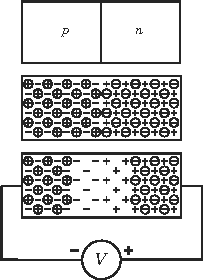
\includegraphics[width=.4\linewidth]{Images/LGADs/p-n junction with voltage.png}
%     \caption{Top: adjacent regions of $p$-doping (left) and $n$-doping forming a $pn$-junction. Middle: the circled mobile charges (holes for $p$-type and electrons for $n$-type) balanced by the charge of atomic cores. Bottom: When an external (reverse) voltage is applied to the central region an electric field builds up in the junction.}
% \end{SCfigure}

%%% WRAPPED FIGURE
% \begin{wrapfigure}{l}{.45\linewidth}
%     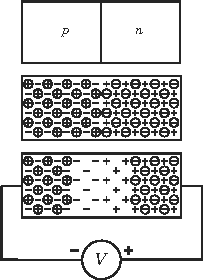
\includegraphics[width=1\linewidth]{Images/LGADs/p-n junction with voltage.png}
%     \caption{Top: adjacent regions of $p$-doping (left) and $n$-doping forming a $pn$-junction. Middle: the circled mobile charges (holes for $p$-type and electrons for $n$-type) balanced by the charge of atomic cores. Bottom: When an external (reverse) voltage is applied to the central region an electric field builds up in the junction.}
%     \label{fig:p-n_junction_reverse_bias_voltage}
% \end{wrapfigure}

%%% FIGURE WITH MINIPAGE
\begin{figure}[!h]
    \begin{minipage}[c]{.25\linewidth}
        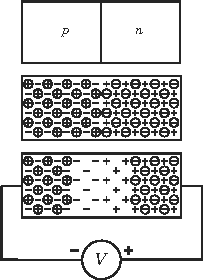
\includegraphics[width=1\linewidth]{Images/LGADs/p-n junction with voltage.png}
    \end{minipage}
    \hfill
    \begin{minipage}[c]{.6\linewidth}
        \caption{\\Top: adjacent regions of $p$-doping (left) and $n$-doping (right) forming a $pn$-junction.\\
        Middle: the circled mobile charges (holes for $p$-type and electrons for $n$-type) balanced by the charge of atomic cores.\\
        Bottom: When an external (reverse) voltage is applied to the junction an electric field builds up in the central region \cite{10.1093/acprof:oso/9780198527848.003.0001}.}
    \end{minipage}
    \label{fig:p-n_junction_reverse_bias_voltage}
\end{figure} 

When a charged particle traverses this depletion layer it frees up electron-hole pairs, which move to the electrodes and can be measured. 

\section{Low Gain Avalanche Detectors}

A particular type of silicon sensors are Low Gain Avalanche Detectors (LGAD), an example is shown is shown in Figure \ref{fig:LGADs_schema}. The major innovation is an additional $p$-type layer below the $n+$ electrode, this creates a high electric field region which leads to an avalanche effect\footnote[2]{When electrons acquire enough energy they can create new electron-hole pairs ('impact ionization'), which can themselves create new pairs and initialize a multiplication chain that leads to an enhanced signal} of the electrons. This effect produces a gain of around $~10$ \marginpar{\flushleft source} 

\begin{figure}[!ht]
    \centering
    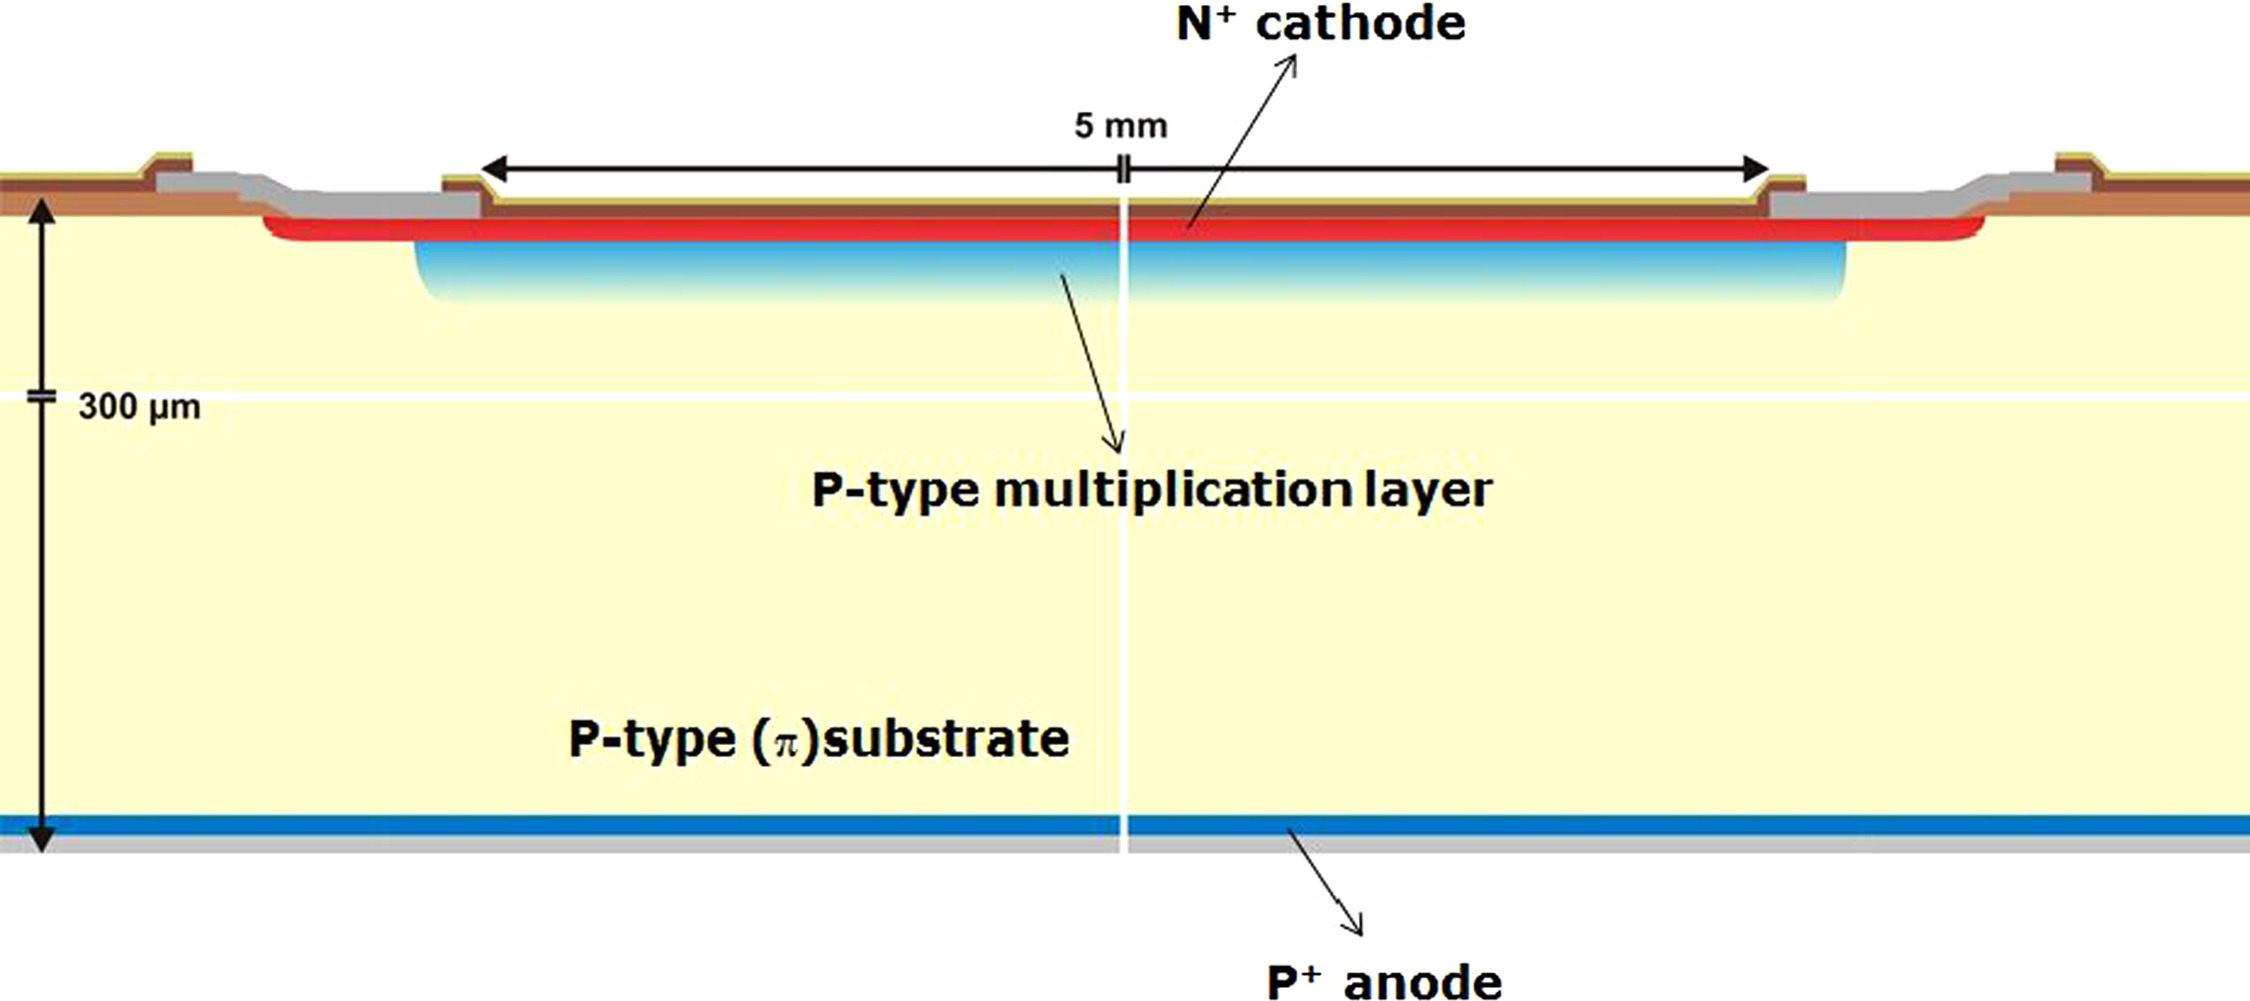
\includegraphics[width=.9\linewidth]{Images/LGADs/1-s2.0-S0168900214007128-gr1_lrg.jpg}
    \caption{description of LGAD}
    \label{fig:LGADs_schema}
\end{figure}

\section{The sensors}
There were several samples that were tested, divided into three main categories of design:
\begin{itemize}
    \item USTC, from the University of Science and Technology of China
    \item IHEP, from the Institute of High Energy Physics, China
    \item CNM, from the Centro National de Microelectronica, Barcelona, Spain
\end{itemize}

the first two designs have both been manufactured by the IME (Institute of Microelectronics) of the Chinese Academy of Sciences. The two CNM sensors (labeled CNM-W4 and CNM-W5) were used to measure the time resolution of another device, the MCP (Section \ref{sec:MCP_description}), which was used as a time reference for all of the time measurements of the other LGADs. Table \ref{tab:devices_tested} provides the list of the devices that were characterized, for more detailed descriptions see Table in \nameref{chap:appendix}.

\begin{table}[!ht]
    \centering
    \caption{Summary of the tested devices}
    \label{tab:devices_tested}
    \scriptsize
    % \makebox[1\textwidth][c]{
    \begin{tabularx}{1\textwidth}{|l|l|l|l|l|X|}
    \hline %%% I NEED TO TRY TO USE TABULAR INSTEAD OF SHORTSTACK
        \textbf{Sevice name} & \textbf{Vendor} & \begin{tabular}{@{}l@{}}\textbf{Pads,} \\ \textbf{used channels}\end{tabular} & \begin{tabular}{@{}l@{}}\textbf{Fluence} \\ $[n_{eq}/\si{cm^2}]$ \end{tabular} & \begin{tabular}{@{}l@{}} \textbf{Radiation} \\ \textbf{type} \end{tabular} & \textbf{Notes} \\
        \hline
        CNM-W4  & CNM & single & 0 & - & reference \\ 
        CNM-W5  & CNM & single & 0 & - & reference \\ 
        CNM-W5-1.5E15  & CNM & single & $\num{1.50E+15}$ & neutron &  \\ 
        CNM-W3-2.5E15  & CNM & single & $\num{2.50E+15}$ & neutron &  \\ 
        USTC2.1-W17 & USTC & 2x2, 2 channels  & 0 & - &  \\ 
        USTC2.1-W17-2E14 & USTC & 2x2, 1 channel & 0 & - & missing \\ 
        IMEv3-W12-2x2  & IHEP & 2x2, 2 channels  & 0 & - &  \\ 
        IMEv3-W12-1x3  & IHEP & 1x3, 2 channels  & 0 & - &  \\ 
        IMEv3-W12  & IHEP & 2x2, 3 channels  & $\num{1.50E+15}$ & neutron &  \\ 
        IMEv3-W16  & IHEP & 1x3, 1 channel  & $\num{1.50E+15}$ & neutron &  \\ 
        IMEv2-W7-1E14  & IHEP & single & $\num{1.00E+14}$ & proton &  \\ 
        IMEv2-W7-6.5E14  & IHEP & single & $\num{6.50E+14}$ & proton &  \\ 
        IMEv3-W16-8E14  & IHEP & single & $\num{8.00E+14}$ & proton &  \\
        IMEv3-W16-2.5E15  & IHEP & single & $\num{2.50E+15}$ & neutron &  \\ 
        \hline
    \end{tabularx}
\end{table}




%%% NOT UPDATED ANYMORE, LOOK AT THE EXCEL FILE, I MIGHT DELETE THIS LATER
%%% I have to reorganize these and associate them with the more accurate descriptions
% device name:        vendor:        sensor ID:            fluence:    irradiation type:    type:        board name:    channels:
% CNM-W4              CNM          CNM-R15973-W4-D168      unirradiated      -             single pad     JSI-B12      1
% CNM-W5              CNM          CNM-R15973-W5-D138      unirradiated      -             single pad     JSI-B14      1
% CNM-W3-2.5E15       CNM          CNM-R15973-W3-D29       $\num{2.5e15}     neutron       single pad     JSI B5       1
% CNM-W5-1.5E15       CNM          CNM-R15973-W5-D29       $\num{1.5e15}     neutron       single pad     JSI PP1      1
% USTC2.1             USTC         USTC2.1-W17-P6-A          0                -             2x2           CERN-3       1,2
% USTC2.1 IRRADIATED (MISSING)
% IMEv3-W12-C2         IHEP        IMEv3-W12-C2-2-2          0               -              2x2          CERN-1       channels 1,2
% IMEv3-W12-C3         IHEP        IMEv3-W12-C3-1-4 (and 5)  0               -              1x3          CERN-1       channles 3,4  (small GR), bonded
% CERN2-CH0-IMEv3-W12  IHEP        IMEv3-W12-B2-2-9-1       1.5e15           neutron        2x2 sensor    CERN-2       channels 1,2,3
% CERN2-CH1-IMEv3-W12  IHEP 
% CERN2-CH2-IMEv3-W12  IHEP 
% CERN2-CH4-IMEv3-W16  IHEP        IMEv3-W16-Q4-D4-1-4      1.5e15           neutron        1x3          CERN-2       channel:  2(?)
% JSI-B6-IMEv2-W7-1E14    IHEP       W7-II-C2-1-7 IMEv2-W7Q2    1e14          proton        single       JSI-B6
% JSI-PP4-IMEv2-W7-6.5E14 IHEP       W7-II-C2-1-7 IMEv2-W7Q2    6.5e14        proton        single       JSI-PP4
% JSI-B7-IMEv3-W16-8E14   IHEP       IHEP-IMEv3-W16_Q4_D3_1-4   8e14          (unsure)        single       JSI-B7
% JSI-B13-IMEv3-W16-2.5E15 IHEP      IHEP-IMEv3-W16_Q4_E3_1-4   2.5e15       (unsure)      single        JSI-B13
                 